%% LyX 2.3.6.1 created this file.  For more info, see http://www.lyx.org/.
%% Do not edit unless you really know what you are doing.
\documentclass[british]{article}
\usepackage[T1]{fontenc}
\usepackage[latin9]{inputenc}
\usepackage{geometry}
\geometry{verbose,tmargin=2cm,bmargin=2cm,lmargin=1cm,rmargin=1cm}
\usepackage{float}
\usepackage{amsmath}
\usepackage{amsthm}
\usepackage{graphicx}
\usepackage{setspace}
\doublespacing

\makeatletter
%%%%%%%%%%%%%%%%%%%%%%%%%%%%%% User specified LaTeX commands.
\usepackage{indentfirst}
\usepackage{mathtools}

\makeatother

\usepackage{babel}
\begin{document}
\title{Molecular Dynamics}
\author{Leonardo H�gens and Johanna L�mker}
\maketitle

\section{Methods}

Molecular Dynamics simulations consist in numerically integrating
the equations of motion of a system, starting from an initial configuration,
and measuring time averages of quantities of interest.

\subsection{Initial Conditions}

Our system consists of $N$ particles in a cubic box $\left[0,L\right]^{3}$,
which gives a particle density of $\rho=\frac{N}{L^{3}}$. The initial
positions where chosen at random with uniform probability inside the
box.

For initial velocities, we first generate every velocity component
randomly with uniform distribution in the interval $\left[-1,1\right]$.
We then calculate the total momentum $\boldsymbol{P}$, and shift
all the velocities equally such that the new total momentum is $0$.
Then, we rescale every velocity component by the same constant such
that the total kinetic energy matches the desired temperature at which
we want to perform our simulation:
\[
E_{kin}=\sum_{i=1}^{N}\frac{mv_{i}^{2}}{2}=\frac{3Nk_{B}T}{2}.
\]


\subsection{Particle Interaction}

We consider the Lennard-Jones potential energy between every pair
of particles, given by:
\[
u\left(r_{ij}\right)=\left\{ \begin{array}{ll}
4\epsilon\left[\left(\frac{\sigma}{r_{ij}}\right)^{12}-\left(\frac{\sigma}{r_{ij}}\right)^{6}\right]-e_{\mathrm{cut}} & r_{ij}\leq r_{\mathrm{cut}}\\
0 & r_{ij}>r_{\mathrm{cut}}
\end{array}\right.,
\]

where
\[
e_{\mathrm{cut}}=4\epsilon\left[\left(\frac{\sigma}{r_{\mathrm{cut}}}\right)^{12}-\left(\frac{\sigma}{r_{\mathrm{cut}}}\right)^{6}\right]
\]

and $r_{\mathrm{cut}}$ is the maximum distance two particles can
have from each other to still be affected by each other's potential.
In our simulations, we set $r_{\text{cut}}=\frac{L}{3}$. 

To obtain the force, we determine the gradient of this potential,
which gives:

\[
\boldsymbol{f}_{ij}=-\nabla u=\left\{ \begin{array}{ll}
-48\frac{\boldsymbol{r}_{ij}}{r_{ij}^{8}}\left(\frac{1}{r_{ij}^{6}}-\frac{1}{2}\right) & r_{ij}\leq r_{\mathrm{cut}}\\
0 & r_{ij}>r_{\mathrm{cut}}
\end{array}\right.,
\]


\subsection{Integration Scheme}

The integration scheme we used in this assignment is the \emph{Velocity
Verlet} algorithm, whose recursive process for each particle goes
as follows, given it's position $\boldsymbol{r}\left(t\right)$, velocity
$\boldsymbol{v}\left(t\right)$ and force acting on it $\boldsymbol{f}(t)$:
\begin{align*}
\boldsymbol{r}(t+dt) & =\boldsymbol{r}\left(t\right)+\boldsymbol{v}\left(t\right)dt+\frac{\boldsymbol{f}(t)}{2m}dt^{2}\\
\boldsymbol{v}\left(t+dt\right) & =\boldsymbol{v}\left(t\right)+\frac{1}{2m}\left(\boldsymbol{f}(t)+\boldsymbol{f}(t+dt)\right)
\end{align*}

We also apply periodic boundary conditions, not only implicitly in
the calculation of the force but also explicitly in the position updates
(apply them when a particles falls outside the box), such that all
positions are always inside the box.

\subsection{NVE and NVT}

For the NVE ensemble, we just run the simulation as described above,
storing $E_{kin}$and $E_{potential}$ at every time step. For the
NVT ensemble, we define a frequency $\nu$, and at every time step
select each particle with probability $\nu\,dt$ to `undergo a collision
with a heat bath at temperature $T$', which in practice means setting
its component's values to randomly generated ones according to the
Maxwell-Boltzmann distribution:
\[
f\left(v_{i}\right)=\sqrt{\frac{m}{2}\frac{\beta}{\pi}}e^{-\frac{m}{2}\beta v_{i}^{2}},
\]

which is a gaussian distribution with mean $\mu=0$ and standard deviation
$\sigma=\frac{1}{\beta m}$. 

More specifically, right after we perform the a verlet step, we generate
a random number in $[0,1]$ with uniform probability, and if it less
than the Andersen probability $\nu\,dt$ we update that particles
velocity components, each with a random value according to $f\left(v_{i}\right)$.

\subsection{Autocorrelation and Diffusion}

The velocity autocorrelation function for a given time difference
$\Delta t$ is evaluated, for $N$ particles, and a run of length
$T$, is given by:
\[
\chi\left(\Delta t\right)=\frac{1}{N}\sum_{i=1}^{N}\frac{1}{T-\Delta t}\sum_{t=1}^{T-\Delta t}\boldsymbol{v}_{i}\left(t\right).\boldsymbol{v}_{i}\left(t+\Delta t\right)
\]

With it, the diffusion coefficient $D$ is given by the Green-Kubo
relation, where $d$ is the system's dimensionality (3 in our case):
\[
D=\frac{1}{d}\int_{0}^{\infty}dt\,\chi\left(t\right)
\]


\section{Results}

\subsection{NVE ensemble}

In our first NVE simulations, we we're using $L=5$ or $L=10$ and
$N=100$, which created some divergences in $E_{\text{kin}}$ and
$E_{pot}$. Of course this was due to the average distance between
particles in this configuration being too small, being easy for two
particles to be too close (and thus have a huge potential energy)
either right at the start of the simulation, when positions are generated
randomly, or at any other instant of the simulation. Thus, we thought
the most sensible thing to do was to use a higher $L$ and low density,
to minimize the possibility of two particles being generated too close
to each other at the start. We also used a not very high temperature,
such that initial velocities are not too high, which prevents particles
from colliding so fast that would make our time step of $dt=0.001$
too high. Thus, we changed to $L=25$, which gives density of $\rho=0.0064$.

\begin{figure}[H]
\begin{centering}
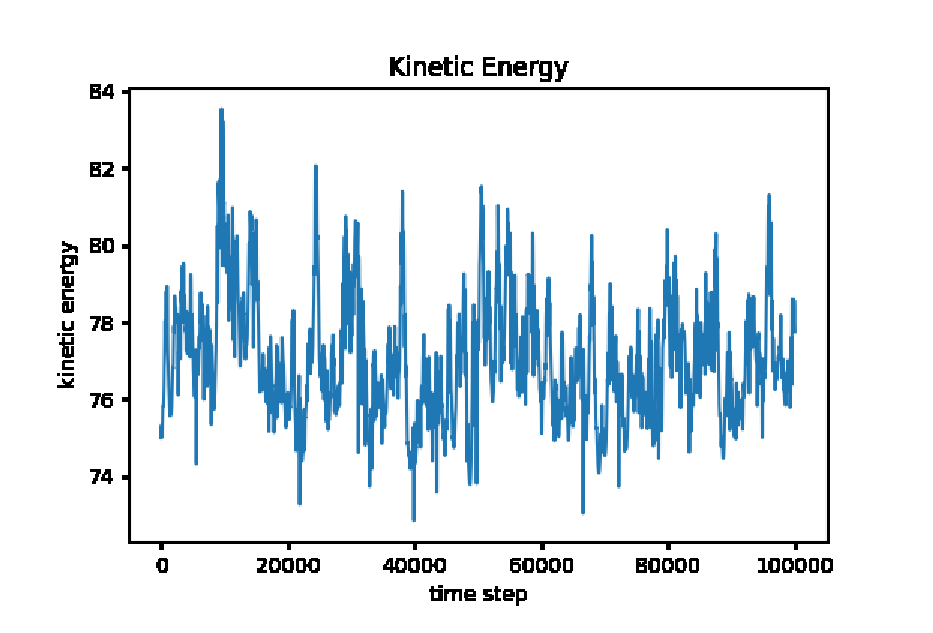
\includegraphics[width=0.5\textwidth]{/home/hugens/shared/uni/modsim/modsim/molecular_dynamics/NVE_results/NVE_kinetic}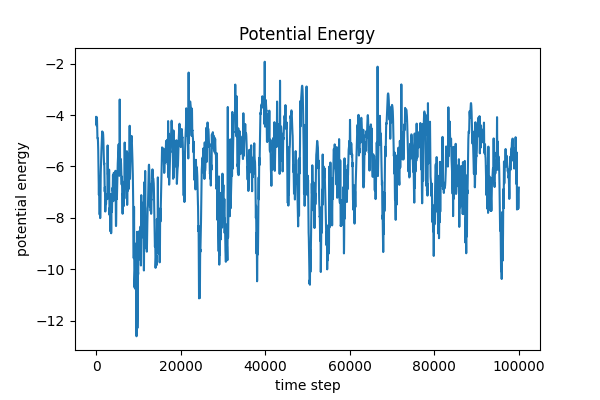
\includegraphics[width=0.5\textwidth]{/home/hugens/shared/uni/modsim/modsim/molecular_dynamics/NVE_results/NVE_potential}
\par\end{centering}
\caption{$E_{\text{kin}}$ and $E_{pot}$ values for the NVE ensemble, with
$N=100$, $\beta=2$, $\rho=0.0064$, $L=25$}
\end{figure}

Let's analyze the plots above. Firstly, we have a visual confirmation
that the way we initialized the velocities is correct, because the
$E_{\text{kin}}$ initial value should be $\frac{3}{2}\frac{N}{\beta}$,
which is 75 for the values we used for $N$ and $\beta$, and that
is exactly the starting value that we see in the plot. Secondly, we
can see roughly see that $E_{\text{kin}}$ and $E_{pot}$ have opposed
behaviors, which is to expect from the NVE ensemble, because it's
what we'd expect from a constant total energy. This is confirmed by
the plot below, where we see that the total energy has a very low
fluctuation in percentage around a value which is $\approx70.93$.
We can also see that the values of $E_{pot}$ are negative. For $N=100$,
this implies not all particles are separated from each other by a
distance in the `sweet spot' range where the potential energy has
a minimum, but most of them are, which makes sense since the initial
velocities are low enough for the particles to converge to those spots
instead of heading onto each other quickly and bouncing back outside
that range.

\begin{figure}[H]
\begin{centering}
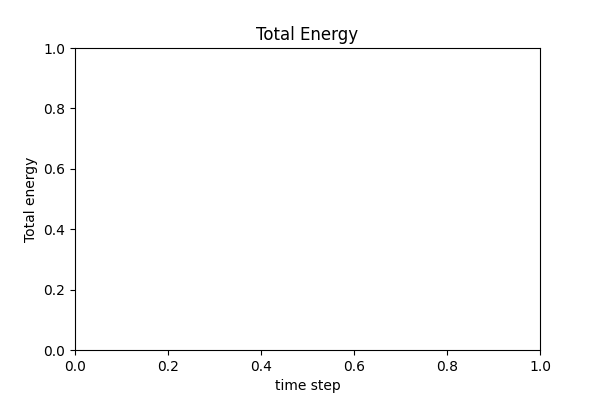
\includegraphics[width=0.6\textwidth]{/home/hugens/shared/uni/modsim/modsim/molecular_dynamics/NVE_results/NVE_total}
\par\end{centering}
\caption{Total Energy values for the NVE ensemble, with $N=100$, $\beta=2$,
$\rho=0.0064$, $L=25$}
\end{figure}


\subsection{NVT ensemble}

For the NVT ensemble, we first wanted to check if the thermostat was
working correctly, so firstly we generated a lot of samples with the
Maxwell Boltzmann distribution we intended to use in the simulations
and plotted a normalized histogram of the samples, which came out
as desired, represented in the Figure below:
\begin{figure}[H]
\begin{centering}
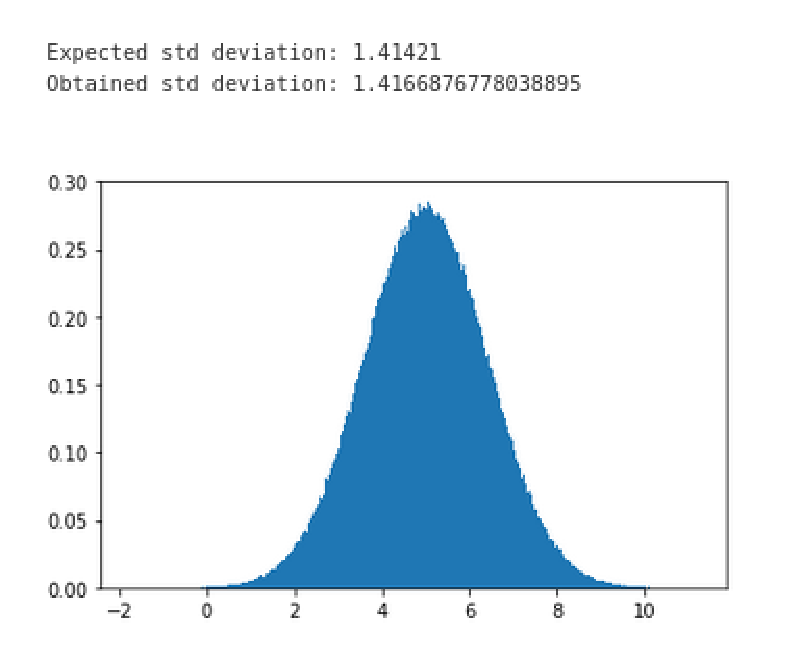
\includegraphics[width=0.6\textwidth]{boltzmann}
\par\end{centering}
\caption{Maxwell-Boltzmann histogram}
\end{figure}

Secondly, we wanted to make sure that per time step $N\,\nu\,dt$
particles where chosen by the thermostat to change their velocity
to a Boltzmann one, so we performed a simulation and plotted the average
number of particles, which also came out as desired:

\begin{figure}[H]
\begin{centering}
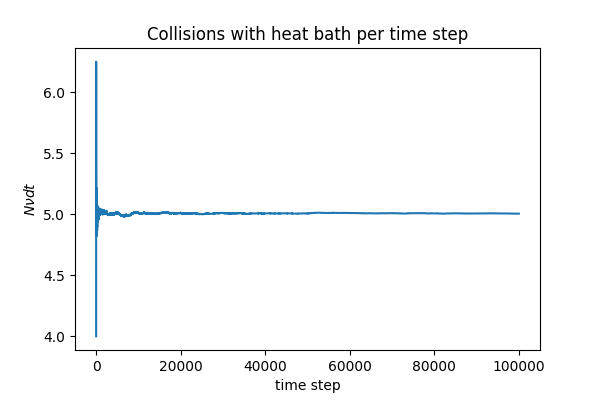
\includegraphics[width=0.6\textwidth]{/home/hugens/shared/uni/modsim/modsim/molecular_dynamics/NVT_results/NVT_thermostat}
\par\end{centering}
\caption{Average number of particles colliding with the heat bath per time
step, with $N=100$, $\nu=50$, $dt=0.001$}
\end{figure}

Running the simulations, we obtained the following curves for $E_{\text{kin}}$
and $E_{pot}$:

\begin{figure}[H]
\begin{centering}
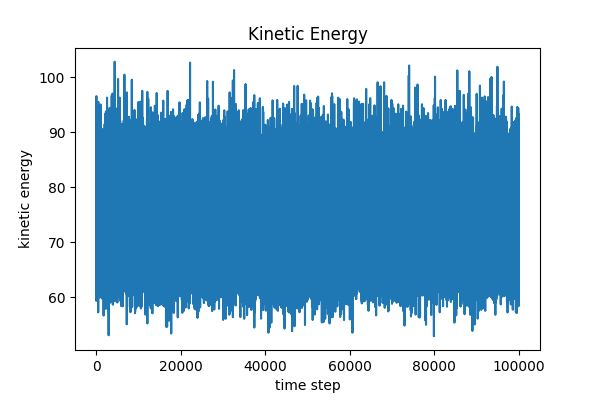
\includegraphics[width=0.5\textwidth]{/home/hugens/shared/uni/modsim/modsim/molecular_dynamics/NVT_results/NVT_kinetic}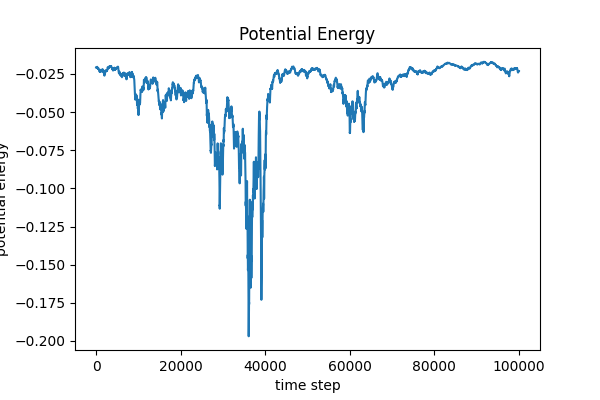
\includegraphics[width=0.5\textwidth]{/home/hugens/shared/uni/modsim/modsim/molecular_dynamics/NVT_results/NVT_potential}
\par\end{centering}
\caption{$E_{\text{kin}}$ and $E_{pot}$ values for the NVT ensemble, with
$N=100$, $\beta=2$, $\rho=0.0064$, $L=25$, $\nu=50$}
\end{figure}

We can observe that $E_{\text{kin}}$ oscillates around the value
$75$, which makes sense since that is the value we determined for
the initial $E_{\text{kin}}$, according to $E_{kin}=\frac{3Nk_{B}T}{2}$.
Because $E_{\text{kin}}$ only differs from the temperature $T$ by
a factor which is constant along the simulation, we can thus verify
with confidence that the thermostat is working, i.e. is keeping the
temperature roughly constant around the desired value. With the thermostat
on, energy is not conserved, which means there is not direct observation
we can make that relates our $E_{\text{kin}}$ curve with our $E_{\text{pot}}$
curve. Because of this lack of evident correlation, we don't think
there is anything important to say about our total energy curve, represented
below.

\begin{figure}[H]
\begin{centering}
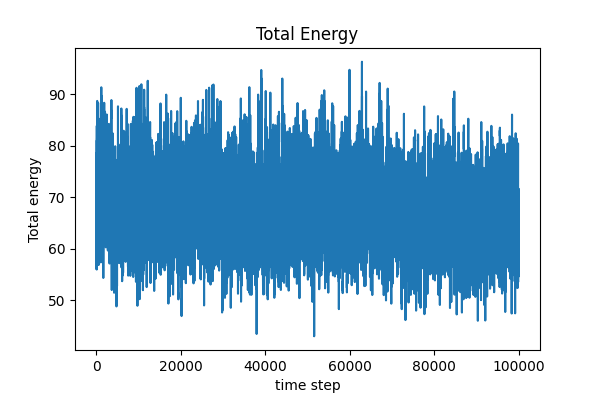
\includegraphics[width=0.6\textwidth]{/home/hugens/shared/uni/modsim/modsim/molecular_dynamics/NVT_results/NVT_total}
\par\end{centering}
\caption{Total Energy values for the NVT ensemble, with $N=100$, $\beta=2$,
$\rho=0.0064$, $L=25$, $\nu=50$}
\end{figure}


\subsection{Diffusion}

\subsubsection{NVE}

Below we represent the velocity autocorrelation function we obtained
for the NVE ensemble simulation to which the plots in the NVE section
refer to. 

\begin{figure}[H]
\begin{centering}
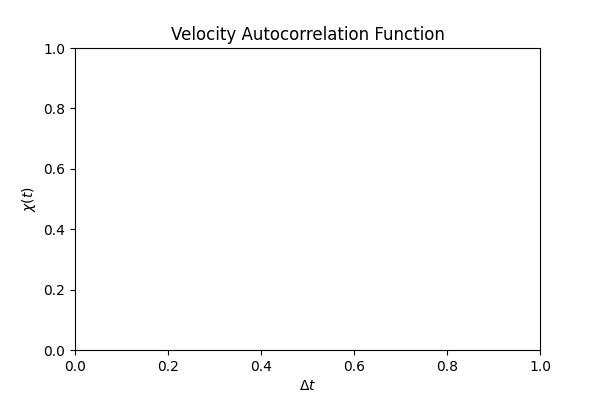
\includegraphics[width=0.5\textwidth]{/home/hugens/shared/uni/modsim/modsim/molecular_dynamics/NVE_results/NVE_vacf}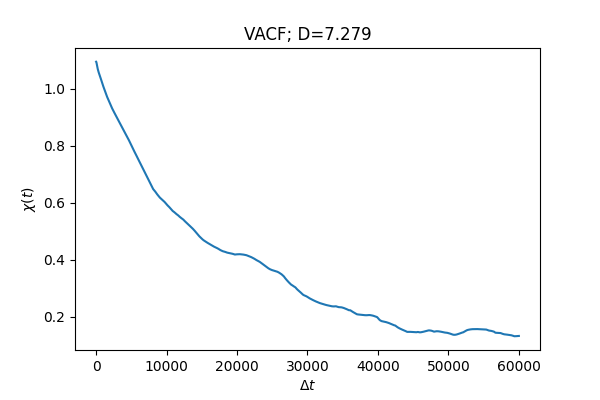
\includegraphics[width=0.5\textwidth]{/home/hugens/shared/uni/modsim/modsim/molecular_dynamics/NVE_results/NVT_vacf_better}
\par\end{centering}
\caption{Velocity autocorrelation function for NVE ensemble, with $N=100$,
$\beta=2$, $\rho=0.0064$, $L=25$}
\end{figure}

An important feature of the correlation function is that when two
consecutive system configurations are highly correlated, as we had
in the Ising single flip procedure, and as we have here, because the
verlet procedure is completely deterministic and two consecutive system
configurations are very similar. In those cases, as it is mentioned
in the Ising notes, an autocorrelation function goes approximately
as $e^{-t/\tau}$, and we think the first part of our plot, roughly
until $t=60000$, highly resembles that curve, as we can see in the
left curve. We find it a bit odd that that first part is compatible
with what we expected, by the previous argument, and then the autocorrelation
shows negative values. 

Firstly, we can argue that as $\Delta t$ approaches the total simulation
time $T$, the sum used to determine the correlation function starts
having less and less terms (e.g. for $\Delta t=T$, only value per
particle is used), and thus the values around that final range start
having less and less statistical significance. However, we also think
it could be related to the average time a particle needs for it to
have enough close encounters with other particles such that it reverts
the direction of it's velocity vector, which would produce negative
terms in the correlation calculation. 

As far as the diffusion constant goes, the full run gives us $D\approx2.773$,
and the `statistically relevant' part gives us $D\approx7.279$.

\subsubsection{NVT}

Below we represent the velocity autocorrelation function we obtained
for the NVT ensemble simulation to which the plots in the NVT section
refer to. 

\begin{figure}[H]
\begin{centering}
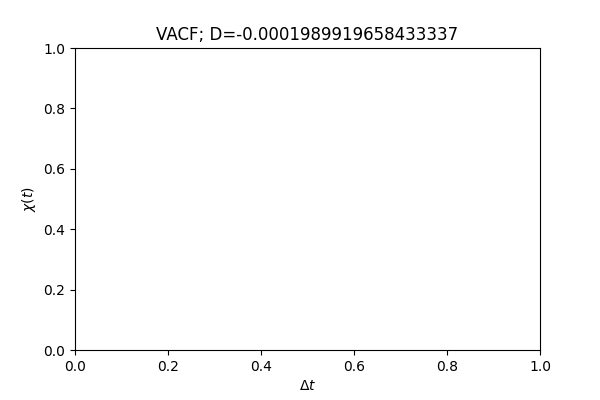
\includegraphics[width=0.6\textwidth]{/home/hugens/shared/uni/modsim/modsim/molecular_dynamics/NVT_results/NVT_vacf}
\par\end{centering}
\caption{Velocity autocorrelation function for the NVT ensemble, with $N=100$,
$\beta=2$, $\rho=0.0064$, $L=25$, $\nu=50$}
\end{figure}

When the Andersen thermostat is switched on, when a certain particle
is chosen to undergo a collision with the heat bath, it's velocity
becomes completely uncorrelated with it's previous velocities, as
its component values are changed to randomly generated ones. In our
simulation, approximately $5$ out of the $100$ particles undergo
this collision per time step, so in average $20$ time steps are needed
for every particle's velocity to have completely lost correlation
with it's previous velocities, which is very little in the scale of
the entire simulation. In the plot, we can see that the autocorrelation
drops from $1.5$ to $0$ almost abruptly, and from there it's stays
pretty much constant, which is completely compatible with the previous
argument. Another important thing we can observe is that the autocorrelation
starts to `falsely' enlarge as $\Delta t$ approaches $T$, which
just comes in handy to support the argument of lack of statistical
significance we gave before, for the NVE ensemble.
\end{document}
